\section{Methodology}\label{sec:methodology}
\subsection{Sensor Node}
Fig.~\ref{fig:system} shows the node. A PIR detector, a carbon dioxide sensor and a sound-level meter are sampled once per second by a microcontroller with 256~kB of flash memory and 64~kB of RAM. The node keeps the last 60~samples of each sensor, runs the network once a minute and sends the result to the building controller over a low-power radio link. Only the estimate leaves the room.

\begin{figure}[t]
  \centering
  % Replace with your own figure: upload an image and change the file name below.
  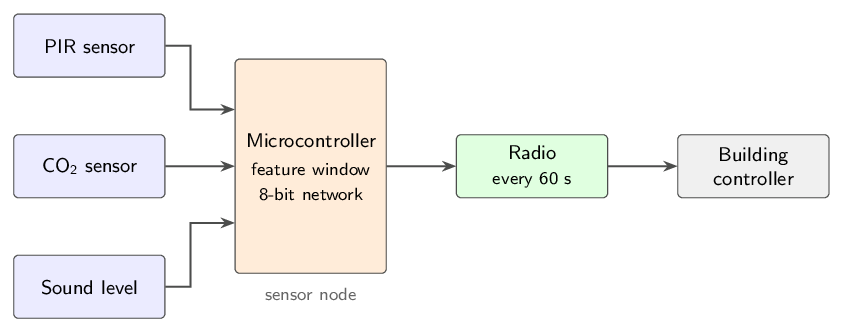
\includegraphics[width=\linewidth]{figures/system-overview.png}
  \caption{The sensor node. Three sensors feed a feature window on the microcontroller; one estimate per minute is sent to the building controller.}
  \label{fig:system}
\end{figure}

\subsection{Network}
The input is a $3 \times 60$ window $\mathbf{x}$ holding one minute of readings from each sensor, normalized per channel. Two depthwise-separable convolution layers with 16 and 24 filters are followed by global average pooling and a fully connected layer with five outputs, one for each occupancy class from empty to four or more people. The model has 4.1~thousand parameters.

\subsection{Training Objective}
Counting errors are not equally costly: confusing two people with three matters less than confusing an empty room with an occupied one. We therefore train with a weighted cross-entropy loss
\begin{equation}\label{eq:loss}
  \mathcal{L}(\theta) = -\frac{1}{N} \sum_{i=1}^{N} w_{y_i} \log p_\theta(y_i \mid \mathbf{x}_i) + \lambda \lVert \theta \rVert_2^2 ,
\end{equation}
where $y_i$ is the true class of window $\mathbf{x}_i$, $w_{y_i}$ is the weight of that class, and $\lambda$ controls weight decay. We set $w_0 = 2$ for the empty class and $w_c = 1$ otherwise, and minimize \eqref{eq:loss} with Adam~\cite{kingma2015adam}.

\subsection{Quantization}
After 40~epochs of floating-point training, weights and activations are constrained to 8-bit integers and the model is trained for ten further epochs so that it adapts to the rounding. Algorithm~\ref{alg:inference} lists the steps the node performs every minute.

\begin{algorithm}[t]
\caption{Occupancy estimate on the node, run once per minute}
\label{alg:inference}
\begin{algorithmic}[1]
\Require buffers $B_{\mathrm{pir}}, B_{\mathrm{co2}}, B_{\mathrm{snd}}$ of 60 samples; quantized network $f_\theta$
\Ensure occupancy class $\hat{y} \in \{0, 1, 2, 3, 4\}$
\State $\mathbf{x} \gets \Call{Normalize}{B_{\mathrm{pir}}, B_{\mathrm{co2}}, B_{\mathrm{snd}}}$
\State $\mathbf{p} \gets f_\theta(\mathbf{x})$ \Comment{38 ms on the microcontroller}
\State $\hat{y} \gets \arg\max_c \, p_c$
\If{$\hat{y} \neq \hat{y}_{\mathrm{prev}}$ \textbf{or} 10 minutes since last transmission}
  \State \Call{Transmit}{$\hat{y}$}
  \State $\hat{y}_{\mathrm{prev}} \gets \hat{y}$
\EndIf
\State sleep until the next minute
\end{algorithmic}
\end{algorithm}
